% $Id: TimeMgmt_refdoc.tex,v 1.1 2002/11/14 23:52:32 jwolfe Exp $

\documentclass[]{article}

\usepackage{epsf}
\usepackage{html}
\usepackage[T1]{fontenc}

\textwidth 6.5in
\textheight 8.5in
\addtolength{\oddsidemargin}{-.75in}

\begin{document}

\bodytext{BGCOLOR=white LINK=#083194 VLINK=#21004A}

\begin{titlepage}

\begin{center}
{\Large Earth System Modeling Framework } \\
\vspace{.25in}
{\Large {\bf Time Management Library F90 Reference}} \\
\vspace{.25in}
{\large {\it Brian Eaton, Cecelia DeLuca, David Neckels, Noel Jorden}}
\vspace{.5in}
\end{center}

\begin{latexonly}
\vspace{5.5in}
\begin{tabular}{p{5in}p{.9in}}
\hrulefill \\
\noindent {\bf NASA High Performance Computing and Communications Program} \\
\noindent Earth and Space Sciences Project \\
\noindent CAN 00-OES-01 \\
\noindent http://www.esmf.ucar.edu \\
\end{tabular}
\end{latexonly}

\end{titlepage}

\tableofcontents

\newpage
%\section{Synopsis}
% $Id: TimeMgmt_syn.tex,v 1.1 2002/11/14 23:55:26 jwolfe Exp $
\section{Synopsis}

The Earth System Modeling Framework (ESMF) Time Management Library provides utility functions for time and date calculations, and higher-level functions that control model time stepping and alarms.  










The design of this Time Management Library is based on the time management 
utilities in the \htmladdnormallink{Flexible Modeling System}{http://www.gfdl.gov/~fms} (FMS) from the 
\htmladdnormallink{NOAA Geophysical Fluid Dynamics Laboratory}{http://www.gfdl.gov}.

It is built on infrastructure derived from the \htmladdnormallink{Portable Extensible 
Toolkit for Scientific Computation}{http://www-fp.mcs.anl.gov/petsc/} (PETSc) 
from \htmladdnormallink{Argonne National Laboratory}{http://www-fp.mcs.anl.gov}.

\section{Installation and General Usage}
See the \htmladdnormallink{ESMF User's Guide}{http://www.esmf.ucar.edu/esmf_docs/ESMF_usrdoc/} for installation instructions and a discussion of overall 
usage of the ESMF libraries.

%\section{Architecture}
%\input{TimeMgmt_arch}

\newpage
\section{Time Class}

\subsection{Description}
% $Id: Time_desc.tex,v 1.5 2003/08/14 20:31:43 cdeluca Exp $
\label{sec:Time}

A Time represents a specific point in time.  In order to accommodate
the range of time scales in Earth system applications, Times in
the ESMF can be specified in many different ways, from years to 
nanoseconds.  The Time interface is designed so that you select one or 
more options from a list of time units in order to specify a 
Time. The options for specifying a Time are shown in 
Figure\ref~{fig:TimeOpts}.  

There are Time methods defined for setting and getting a
Time, incrementing and decrementing a Time by a TimeInterval,
taking the difference between two Times, and comparing Times.
Special quantities such as the middle of the month and the 
day of the year associated with a particular Time can be retrieved. 
There is a method for returning the Time value as a string in 
the ISO 8601 format YYYY-MM-DDThh:mm:ss.

A Time that is specified in hours, minutes, seconds, or subsecond intervals 
does not need to be associated with a standard calendar; a Time whose
specification includes larger units must be.  The ESMF representation
of a calendar, the Calendar class, is described in Section~\ref{sec:Calendar}.
The {\tt ESMF_TimeSet} method can be called to associate a Time with a 
Calendar.  If an operation is requested in which a Calendar is necessary 
and one has not been set, the ESMF method will return an error.

In the ESMF the TimeInterval class used to represent time periods.
This class is frequently used in combination with the Time class.
The Clock class, for example, advances model time by 
 
Times are used by other classes in the ESMF timekeeping system,
 such as Clocks (Section~\ref{sec:Clock}) and Alarms 
(Section~\ref{sec:Alarm}).






\subsection{Restrictions}
% $Id$

\begin{enumerate}

\item {\bf Limits on size and resolution of Time.}  The limits on the size and 
resolution of the time representation are based on the
64-bit integer types used.  For seconds, a signed 64-bit integer
will have a range of +/- $2^{63}$-1, or +/- 9,223,372,036,854,775,807.  This
corresponds to a maximum size of +/- ($2^{63}$-1)/(86400 * 365.25) or
+/- 292,271,023,045 years.

\begin{sloppypar}
For fractional seconds, a signed 64-bit integer will handle a resolution of
+/- $2^{31}$-1, or +/- 9,223,372,036,854,775,807 parts of a second.
\end{sloppypar}

\end{enumerate}


\subsection{Use and Examples}
% $Id: Time_fex.tex,v 1.8 2003/08/29 22:26:14 eschwab Exp $

\begin{verbatim}
use ESMF_Mod

! Create 3 Time instants
type(ESMF_Time) :: startTime1, startTime2, startTime3

! Initialize first to 8/1/2002, 14:25:45.250, Gregorian calendar
call ESMF_TimeSet(startTime1, yr=2002, mm=8, dd=1, &
                  h=14, m=25, s=45, ms=250, gregorian)

! Initialize second to real time (wall clock time)
call ESMF_TimeSyncToRealTime(startTime2)

! Initialize third to be same as second
startTime3 = startTime2

\end{verbatim}


\newpage
\section{Date Class}

\subsection{Description}
% $Id: Date_desc.tex,v 1.1 2002/11/14 23:47:36 jwolfe Exp $

The {\tt Date} class provides a set of functions for manipulating dates.
These include setting and retrieving dates, incrementing and decrementing 
dates by a specified time interval, taking the difference of two dates,
determining whether one date is later than another, and computing the
day of year of a given date.
   
The {\tt Date} class contains attributes representing year, month and day 
quantities and a time of day.  It also contains a calendar which 
stores, for a given year, such quantities as the number of days per 
month and per year.  Gregorian and no-leap year calendars are currently 
supported.  

The algorithm to convert from Gregorian to Julian days is from 
Henry F. Fliegel and Thomas C. Van Flandern, in Communications of 
the ACM (CACM, volume 11, number 10, October 1968, p.657).  Julian 
day refers to the number of days since a reference day.  For the 
algorithm used, this reference day is November 24, -4713 in the Gregorian 
calendar.  The algorithm is valid through all future dates, assuming 
standard corrections are applied (at 4 years, 100 years,
and 400 years).




\subsection{Restrictions}
% $Id: Date_rest.tex,v 1.1 2002/11/14 23:48:55 jwolfe Exp $

The Gregorian date object is limited to the range
November 25, -4713 to December 31, +214748 (both in the Gregorian calendar).  The lower limit
is due to the algorithm used in the Gregorian calendar, which relies on
calculating the julian day.  This calculation is valid only for a positive
julian day, and the lower limit corresponds to the julian day of one.  The
upper limit is imposed because January 1, 214749 is expressed in the {\tt yearmmdd}
format as 2147490101, which is larger than \( 2^{31} \).

The No Leap date object is limited to the range January 1, -214748 to
December 31, +21478 .  Both of these limitations derive from the {\tt yearmmdd}
interface and the fact that the year 21479 (B.C. or A.D.) can not be represented
in this format and a 4-byte integer.





\subsection{Future Plans}
% $Id: Date_fut.tex,v 1.1 2002/11/14 23:48:30 jwolfe Exp $

The current range restrictions for the date object are primarily an artifact of
the {\tt yearmmdd} interface.  The underlying objects are capable of greater ranges.
The upper range of the Gregorian calendar can be extended to October 17, 1465002, 
at which date the julian day calculation overflows.  The current Gregorian lower limit 
can not be changed.

The No-Leap limits can be extended to the years \( 2^{31} \) (A.D) and \( 2^{31} - 1 \) (B.C.).  
They do not suffer the limits placed on the Gregorian calendar by the julian day 
calculation.  They are limited by a 4 byte integer holding the year.

If the ranges imposed by the {\tt yearmmdd} interface are too narrow, the library interface
can change to accomodate a separate integer for each of year, month and day.


\subsection{Use and Examples}
% $Id: Date_fex.tex,v 1.1 2002/11/14 23:48:06 jwolfe Exp $

In the example below we demonstrate basic usage of the {\tt Date} class.  For
a detailed description of the {\tt Date} class interface, see 
Appendix A.

The example shows how to initialize a Gregorian {\tt Date} and increment 
it by a specified time interval.  Since no memory is allocated from the heap
when a {\tt Date} is initialized, there is no need to deallocate a 
{\tt Date} object.

\begin{verbatim}

  use ESMF_TimeMgmtMod

  type(ESMF_Time) :: interval
  type(ESMF_Date) :: startDate, endDate

!-------------------------------------------------------------------------------    
! Initialize a date to July 20, 1998 and 0 seconds. 
!-------------------------------------------------------------------------------

  startDate = ESMF_DateInit(ESMF_GREGORIAN, 19980720, 0) 

!-------------------------------------------------------------------------------    
! Initialize a time to 250 days and 7200 seconds. 
!-------------------------------------------------------------------------------

  interval = ESMF_TimeInit(250, 7200)

!-------------------------------------------------------------------------------    
! Increment the date with the time. 
!-------------------------------------------------------------------------------
       
  endDate = ESMF_DateIncrement(startDate, interval)
\end{verbatim}






\newpage
\section{TimeMgr Class}

\subsection{Description}
% $Id: TimeMgr_desc.tex,v 1.15 2003/09/02 18:42:25 eschwab Exp $

The ESMF Time Manager utility includes software for time and date 
representation and calculations, model time advancement, and the 
identification of unique and periodic events.  Since multi-component 
geophysical applications often require synchronization across
the time management schemes of the individual components, the 
Time Manager's standard calendars and consistent time representation 
promote component interoperability.
\begin{center}  
\begin{tabular}{|p{6in}|}
\hline
\vspace{.01in}
{\bf Key Features} \\[.01in]
Drift-free timekeeping through an integer-based internal time 
representation. \\
The ability to represent time as a rational fraction, to support 
exact timekeeping in applications that involve grid refinement. \\
Support for many calendar types, including user-customized calendars. \\
Support for both concurrent and sequential modes of component execution. \\
Support for varying and negative time steps. \\[.03in] \hline
\end{tabular}
\end{center}

\subsection{Time Manager Classes}
There are five ESMF classes that represent time concepts:
\begin{itemize}
\item {\bf Calendar}  A Calendar can be used to keep track of the 
date as an ESMF Gridded Component advances in time. Standard calendars 
(such as Gregorian and 360-day) and user-specified calendars are 
supported.  Calendars can be queried for quantities such as seconds 
per day, days per month, and days per year.  
\item {\bf Time} A Time represents a time instant in a particular
calendar, such as November 28, 1964, at 7:31pm EST in the Gregorian 
calendar.  The Time class can be used 
to represent the start and stop time of a time integration.
\item {\bf TimeInterval} TimeIntervals represent a period 
of time, such as 300 milliseconds.  Time steps can be represented 
using TimeIntervals.  
\item {\bf Clock} Clocks collect the parameters and 
methods used for model time advancement into a convenient 
package.  A Clock can be queried for quantities such
as start time, stop time, current time, and time step.  Clock
methods include incrementing the current time, and determining
if it is time to stop.  
\item {\bf Alarm} Alarms identify unique or periodic events
by ``ringing'' - returning a true value - at specified times.  
For example, an Alarm might be set to ring on the day of the 
year when leaves start falling from the trees in a climate model.
\end{itemize}

\begin{center}
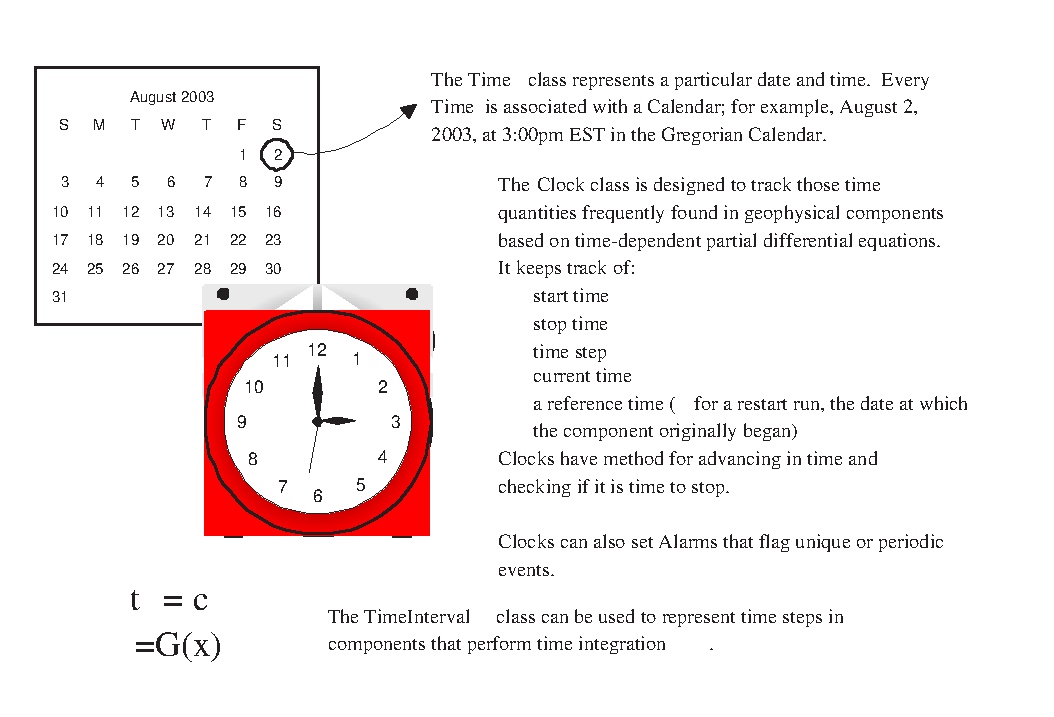
\includegraphics{TimeMgr_desc.eps}
\end{center}

\newpage
In the remainder of this section, we briefly summarize the 
functionality that the Time Manager classes provide.  Detailed 
descriptions and examples of use precede the API listing for each 
class.

\subsection{Calendar}
An ESMF Calendar can be queried for seconds per day, days per month 
and days per year.  The flexible definition of Calendars allows them
to be defined for planetary bodies other than Earth.  The set of supported 
calendars includes:
\begin{description}
\item [Gregorian] The standard Gregorian calendar.
\item [no-leap] The Gregorian calendar with no leap years.
\item [Julian Day] A Julian days calendar.
\item [360-day] A 30-day-per-month, 12-month-per-year calendar.
\item [no calendar] Tracks only timesteps.
\end{description}
See Section~\ref{sec:Calendar} for more details on supported standard 
calendars, and how to create a customized ESMF Calendar.

\subsection{Time Instants and Time Intervals}

TimeIntervals and Time instants (simply called Times) are the computational 
building blocks of the Time Manager utility.  TimeIntervals, which are 
time periods independent of a calendar, support operations such as add, 
subtract, compare size, 
reset value, copy value, and subdivide by a scalar.  Times, which 
are moments in time associated with specific Calendars, can be incremented 
or decremented by TimeIntervals, compared to see which of two Times 
is later, differenced to obtain the TimeInterval between two Times, 
copied, reset, and manipulated in other useful ways.  Times support a 
host of different queries, both for values of individual Time 
components such as year, month, day, and second, and for derived values such 
as day of year, middle of current month and Julian day.  It is also possible 
to retrieve the value of the hardware realtime clock in the form of a 
Time.  See Sections~\ref{sec:Time} and ~\ref{sec:TimeInterval}, respectively,
for use and examples of Times and TimeIntervals.

Since climate modeling, numerical weather prediction and other 
Earth and space applications have widely varying time scales and require 
different sorts of calendars, Times and TimeIntervals must support 
a wide range of time specifiers, spanning nanoseconds to years.  The
interfaces to these time classes are defined so that you can specify a time
using a combination of units selected from the list shown in 
Table~\ref{table:timeOpts}.  

\subsection{Clocks and Alarms}
Although it is possible to repeatedly step a Time forward by a 
TimeInterval using arithmetic on these basic types, it is useful to 
identify a higher-level concept to represent this function.  We refer to 
this capability as a Clock, and include in its required features the 
ability to store the start and stop times of 
a model run, to check when time advancement should cease, 
and to query the value of quantities such as the current time and the
time at the previous time step.  The Time Manager includes a class 
with methods that return a true value when a periodic or unique event 
has taken place; we refer to these as Alarms.  Applications may contain 
temporary or multiple Clocks and Alarms.  Sections~\ref{sec:Clock} and
\ref{sec:Alarm} describe the use of Clocks and Alarms in detail.








\subsection{Use and Examples}
% $Id: TimeMgr_fex.tex,v 1.1 2002/11/14 23:57:36 jwolfe Exp $

The example below demonstrates usage of the {\tt TimeMgr} class.  For
a detailed description of the {\tt TimeMgr} class interface, see 
Appendix A.

We initialize a {\tt TimeMgr} with a start date, an end date, and a timestep.  
The {\tt TimeMgr} advances the model calendar until it recognizes that it is on the last 
timestep.  Since no memory is allocated from the heap when a {\tt TimeMgr} is initialized, 
there is no need to deallocate a {\tt TimeMgr} object.

\begin{verbatim}      

  use ESMF_TimeMgmtMod

  type(ESMF_Time) :: stepSize
  type(ESMF_Date) :: startDate, endDate
  type(ESMF_TimeMgr) :: timeMgr

!-------------------------------------------------------------------------------    
! Initialize the model timestep to 1 day, 1800 seconds; the start date to 
! December 1, 2001 and 0 seconds; and the end date to March 14, 2003 and 
! 0 seconds.  Dates are represented in a YYYYMMDD format.  In this example
! we use a Gregorian calendar. 
!-------------------------------------------------------------------------------

  stepSize = ESMF_TimeInit(1, 1800)
  startDate = ESMF_DateInit(ESMF_GREGORIAN, 20011201, 0)
  endDate = ESMF_DateInit(ESMF_GREGORIAN, 20030314, 0)

!-------------------------------------------------------------------------------    
! Initialize the time manager.
!-------------------------------------------------------------------------------

  timeMgr = ESMF_TimeMgrInit(stepSize, startDate, endDate)

!-------------------------------------------------------------------------------    
! Advance the model until the end date.
!-------------------------------------------------------------------------------

  do while (.NOT. ESMF_TimeMgrLastStep(timeMgr))
    ! Execute model code
    call ESMF_TimeMgrAdvance(timeMgr)
  end do

\end{verbatim}






\newpage
\section{Alarm Class}

\subsection{Description}
% $Id: Alarm_desc.tex,v 1.1 2002/10/08 18:13:09 eschwab Exp $

The Alarm class encapsulates the required alarm behavior, triggering its
ringing state on either a one-shot or repeating interval basis.


\subsection{Use and Examples}
% $Id: Alarm_fex.tex,v 1.8 2003/09/10 23:56:34 eschwab Exp $

\begin{verbatim}
use ESMF_Mod

! create two Alarms
type(ESMF_Alarm) :: alarm1, alarm2

! Initialize one to be a one-shot
type(ESMF_Time) :: alarmTime
call ESMF_TimeSet(alarmTime, yr=2002, mm=8, dd=30, calendar=gregorian)
call ESMF_AlarmSetup(alarm1, ringTime=alarmTime)

! Initialize other to ring on an interval
type(ESMF_TimeInterval) :: alarmInterval
call ESMF_TimeIntervalSet(alarmInterval, dd=1)
call ESMF_AlarmSetup(alarm2, ringInterval=alarmInterval)

! Associate alarms with clock
call ESMF_ClockAddAlarm(modelTime, alarm1)
call ESMF_ClockAddAlarm(modelTime, alarm2)

! Time step, clock reports active alarms in RingingAlarms list
call ESMF_ClockAdvance(modelTime, numRingingAlarms=numActiveAlarms)

! Process any active alarms
type(ESMF_Pointer) :: alarm
do i=1,numActiveAlarms
  call ESMF_ClockGetRingingAlarm(modelTime, i, alarm)
  ! process alarm(i)
  call ProcessAlarm(alarm)  ! user method

 ! after processing alarms, turn off interval alarm to prepare for next
 !   ring time
 call ESMF_AlarmRingerOff(alarm)
end do
\end{verbatim}


%\section{Glossary}
% $Id: TimeMgmt_glos.tex,v 1.1 2002/11/14 23:51:54 jwolfe Exp $
\section{Glossary}

\begin{description}

\item [date] \label{glos:date} A date is used to specify an instant of time at the Greenwich meridian.  It consists
of year, month, day of month and time of day components.

\item [time] \label{glos:time} A time is used to specify an interval of time. 
              
\item [day of year] \label{glos:dayofyear} The day number in the calendar year. January 1 is day 1 of the year. 
Day of year expressed in a floating point format is used to express the day number plus the time of day 
at Greenwich. For example, assuming a Gregorian calendar: 

\begin{tabular}{ll}
{\bf date}              & {\bf day of year} \\
\hline 
10 January 2000, 6Z     & 10.25 \\
31 December 2000, 18Z   & 366.75 
\end{tabular}

\item [no-leap calendar] \label{glos:noleap} Every year uses the same months and days per month as in a non-leap 
year of a Gregorian calendar.

\end{description}













%\section{Bibliography}
%\bibliography{comp} 
%\bibliographystyle{plain}
%\addcontentsline{toc}{section}{Bibliography}

\newpage
\setcounter{section}{1}
\renewcommand{\thesection}{\Alph{section}}
\renewcommand{\thesubsection}{\thesection\arabic{subsection}}

\section*{Appendix A:  Fortran Interface}
\addcontentsline{toc}{section}{Appendix A:  Fortran Interface}

\input{ESMF_TimeMod}

\input{ESMF_DateMod}

\input{ESMF_TimeMgrMod}

\input{ESMF_AlarmMod}

\newpage
\setcounter{section}{2}
\renewcommand{\thesection}{\Alph{section}}
\renewcommand{\thesubsection}{\thesection\arabic{subsection}}

\section*{Appendix B:  Class Implementations}
\addcontentsline{toc}{section}{Appendix B:  Class Implementations}

\subsection{Public Classes}

\input{ESMC_Time}

\input{ESMC_Date}

\input{ESMC_TimeMgr}

\input{ESMC_Alarm}

\subsection{Private Classes}

\input{ESMC_Calendar}

\input{ESMC_TOD}

\end{document}










